\documentclass[compress]{beamer}
\usepackage{multicol}
\usepackage{float}
%\usetheme{Antibes}
\useoutertheme[footline=institutetitle, subsection=true]{miniframes}
\useinnertheme{circles}
\usecolortheme{beaver}
\usefonttheme{structurebold}
\usepackage[utf8]{inputenc}
%\usepackage{titlesec}
\usepackage{amsmath}
\usepackage{mathspec}
%\setcounter{section}{2}
\setcounter{tocdepth}{2}
\usepackage{graphicx}
\usepackage{soul}
\usepackage{hyperref}
%\usepackage[justification=centering]{caption}
\graphicspath{ {./images/} }
\usepackage[backend=biber, citestyle=authoryear, bibstyle=numeric, sorting=none]{biblatex}
\addbibresource{ref.bib}
%\usepackage{fontspec}   %加這個就可以設定字體
\usepackage{xeCJK}       %讓中英文字體分開設置
\setCJKmainfont{Noto Sans CJK TC} %設定中文為系統上的字型
%\newCJKfontfamily[chinesexSerif]\CJKserif{Noto Serif CJK TC}
\setmainfont{Sabon}
\setsansfont{Goldman Sans}
\setmathfont(Digits,Latin){Consolas}
%\usefonttheme[onlymath]{serif}
\setmonofont{Roboto Mono}
\XeTeXlinebreaklocale "zh"             %這兩行一定要加,中文才能自動換行
\XeTeXlinebreakskip = 0pt plus 1pt     %這兩行一定要加,中文才能自動換行
%\renewcommand{\baselinestretch}{1.2}

\title{Measuring the Social Return of Higher Education}
\author{鄭泊聲、倪楷恩、陳致宇、白崇佑}
\institute{國立台灣大學}
\date{\today}

\AtBeginSection[]
{
    
  \begin{frame}[allowframebreaks]
    
    \tableofcontents[currentsection]
    
  \end{frame}
}

\AtBeginSubsection[]{
    \begin{frame}[allowframebreaks]
        \tableofcontents[currentsubsection]
    \end{frame}
}

\begin{document}
\setbeamertemplate{navigation symbols}{\insertframenumber/\inserttotalframenumber}

\begin{frame}
    \titlepage
\end{frame}

\section{The Idea}
\begin{frame}{External versus Internal}
  \begin{itemize}
    \item Government subsides for higher education is high. Is this justified?
    \item Basic demand and supply model tells us: government subside for external benefits maximize welfare.
    \item How can we measure the external benefits?
    \begin{itemize}
      \item Education increases personal wage, but that's \textbf{internal}.
    \item How about average wage in regions with different amount of higher education? This might include \textbf{external} effect. 
    \end{itemize}
    
  \end{itemize}
  Much of this work is based on \cite{MORETTI2004175}.
\end{frame}

\begin{frame}{Data and Variables}
  \begin{itemize}
    \item Wage data: a data based on workplace (instead of household) location city average wage data calculated by DGBAS. Only 2018-2020.
    \item Education data: How to measure "the amount of higher education"?
    \begin{itemize}
      \item No. of college gradutes in city\footnote{Depart. of Statistics, Ministry of Education}
      \item Share of college level worker in city workforce\footnote{縣市重要統計指標查詢系統, DGBAS}
      \item City population education level - above college share \footnote{人口統計資料, Dept. of Household Registration}
    \end{itemize}
    \item Other city characteristic data as controls
  \end{itemize}
\end{frame}

\begin{frame}{}
  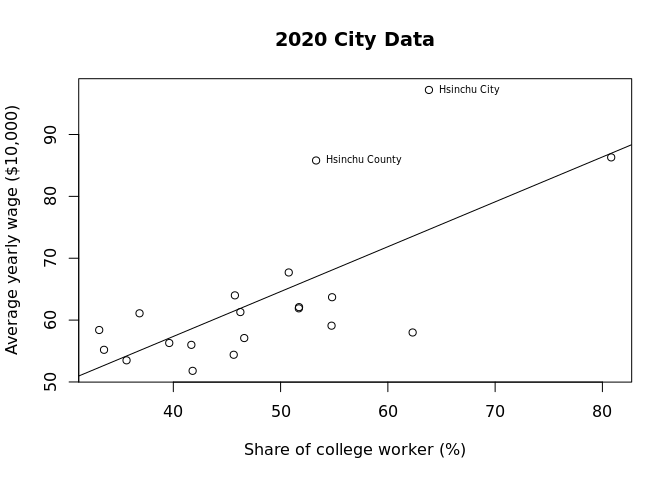
\includegraphics[width=\linewidth]{unnamed-chunk-13-1.png}
\end{frame}

\section[Cross Section]{Cross Sectional MLR}

\begin{frame}{Model Specification}
  Dependent variable is city wage at 2020, $wage2020$. The full MLR model is 
  \begin{equation}
    wage2020 = \beta_0 + workforceCollege\_2020 + \mathbf{\beta X} + u
  \end{equation}
  with $workforceCollege\_2020$, the share of college educated worker in city workforce, as main explanatory. $\mathbf{X}$ is a vector containing
  various city characteristic, including
  \begin{itemize}
    \item $direct$: a dummy for the 6 Special Municipality
    \item $directEdu2020$: a interaction term between $direct$ and $workforceCollege\_2020$ to allow different slope.
  \end{itemize}
\end{frame}

\begin{frame}{All variables}
    \begin{table}[!htbp] \centering \fontsize{5pt}{6pt}\selectfont
        \caption{MLR on all variables} 
        \label{tab: mlr2} 
        \begin{multicols}{2}
            \begin{tabular}{@{\extracolsep{5pt}}lc} 
                \\[-1.8ex]\hline 
                \hline \\[-1.8ex] 
                 & \multicolumn{1}{c}{\textit{Dependent variable:}} \\ 
                \cline{2-2} 
                \\[-1.8ex] & wage2020 \\ 
                \hline \\[-1.8ex] 
                 workforceCollege\_2020 & $-$0.818 \\ 
                  & (1.814) \\ 
                  & \\ 
                 direct & 81.297$^{**}$ \\ 
                  & (23.442) \\ 
                  & \\ 
                 hired2020 & 1.486$^{**}$ \\ 
                  & (0.608) \\ 
                  & \\ 
                 manufecture2020 & $-$2.045$^{**}$ \\ 
                  & (0.850) \\ 
                  & \\ 
                 service2020 & $-$1.049 \\ 
                  & (0.915) \\ 
                  & \\ 
                 gender2020 & 2.499$^{**}$ \\ 
                  & (0.994) \\ 
                  & \\ 
                 eduExpense2020 & 1.162$^{*}$ \\ 
                  & (0.572) \\ 
                  & \\ 
                \end{tabular}
                \begin{tabular}{@{\extracolsep{5pt}}lc} 
                 eduLevel2020 & 1.866 \\ 
                  & (1.746) \\ 
                  & \\ 
                 married2020 & 1.504 \\ 
                  & (1.141) \\ 
                  & \\ 
                 expensePerCapita2020 & 0.003$^{***}$ \\ 
                  & (0.001) \\ 
                  & \\ 
                 unemployment2020 & $-$31.468 \\ 
                  & (21.214) \\ 
                  & \\ 
                 directEdu2020 & $-$1.531$^{***}$ \\ 
                  & (0.416) \\ 
                  & \\ 
                 Constant & $-$268.635 \\ 
                  & (171.289) \\ 
                  & \\ 
                \hline \\[-1.8ex] 
                Observations & 20 \\ 
                R$^{2}$ & 0.959 \\ 
                Adjusted R$^{2}$ & 0.888 \\ 
                Residual Std. Error & 4.055 (df = 7) \\ 
                F Statistic & 13.604$^{***}$ (df = 12; 7) \\ 
                \hline 
                \hline \\[-1.8ex] 
                \textit{Note:}  & \multicolumn{1}{r}{$^{*}$p$<$0.1; $^{**}$p$<$0.05; $^{***}$p$<$0.01} \\ 
                \end{tabular} 
        \end{multicols}
      
      \end{table}
\end{frame}

\begin{frame}{Joint significance of education}
    \begin{table}[!htbp] \centering \tiny
        \caption{} 
        \label{} 
      \begin{tabular}{@{\extracolsep{5pt}}lc} 
      \\[-1.8ex]\hline 
      \hline \\[-1.8ex] 
       & \multicolumn{1}{c}{\textit{Dependent variable:}} \\ 
      \cline{2-2} 
      \\[-1.8ex] & wage2020 \\ 
      \hline \\[-1.8ex] 
       workforceCollege\_2020 & 0.946 \\ 
        & (1.231) \\ 
        & \\ 
       eduExpense2020 & 0.650 \\ 
        & (0.530) \\ 
        & \\ 
       eduLevel2020 & $-$0.333 \\ 
        & (1.259) \\ 
        & \\ 
       Constant & 9.424 \\ 
        & (18.926) \\ 
        & \\ 
      \hline \\[-1.8ex] 
      Observations & 20 \\ 
      R$^{2}$ & 0.525 \\ 
      Adjusted R$^{2}$ & 0.436 \\ 
      Residual Std. Error & 9.118 (df = 16) \\ 
      F Statistic & 5.889$^{***}$ (df = 3; 16) \\ 
      \hline 
      \hline \\[-1.8ex] 
      \textit{Note:}  & \multicolumn{1}{r}{$^{*}$p$<$0.1; $^{**}$p$<$0.05; $^{***}$p$<$0.01} \\ 
      \end{tabular} 
      \end{table} 
\end{frame}

\subsection{College Worker Share}

\begin{frame}{The Model}
  We take only reasonable and strong variables to form a compelling model as
  \begin{multline}
    wage2020 = \beta_0 + \beta_1 workforceCollege\_2020 + \delta_0 direct\\ + \beta_2 wage2018 + \beta_3 manufecture2020 + \beta_4 hired2020
  \end{multline}
  \begin{itemize}
    \item $wage2018$: a lagged dependent as proxy to most of the city characteristics
    \item $manufecture2018$ is the share of manufecturing industry in gross production, $hired2020$ is the share of workforce classified as hired (instead of being employer or self-employed)
  \end{itemize}
\end{frame}

\begin{frame}{MLR}
    \begin{table}[!htbp] \centering \tiny
        \caption{} 
        \label{} 
        \begin{multicols}{2}
          \begin{tabular}{@{\extracolsep{5pt}}lc} 
            \\[-1.8ex]\hline 
            \hline \\[-1.8ex] 
             & \multicolumn{1}{c}{\textit{Dependent variable:}} \\ 
            \cline{2-2} 
            \\[-1.8ex] & wage2020 \\ 
            \hline \\[-1.8ex] 
             workforceCollege\_2020 & 0.075$^{**}$ \\ 
              & (0.029) \\ 
              & \\ 
             direct & $-$0.194 \\ 
              & (0.413) \\ 
              & \\ 
             wage2018 & 1.017$^{***}$ \\ 
              & (0.021) \\ 
              & \\ 
             manufecture2020 & 0.025 \\ 
              & (0.022) \\ 
              & \\ 
             hired2020 & $-$0.032 \\ 
              & (0.038) \\ 
              & \\ 
             Constant & $-$1.259 \\ 
              & (2.005) \\ 
              & \\ 
            \hline \\[-1.8ex] 
          \end{tabular}
          \begin{tabular}{@{\extracolsep{5pt}}lc} \hline \\
            Observations & 20 \\ 
            R$^{2}$ & 0.998 \\ 
            Adjusted R$^{2}$ & 0.997 \\ 
            Residual Std. Error & 0.689 (df = 14) \\ 
            F Statistic & 1,175.873$^{***}$ (df = 5; 14) \\ 
            \hline 
            \hline \\[-1.8ex] 
            \textit{Note:}  & \multicolumn{1}{r}{$^{*}$p$<$0.1; $^{**}$p$<$0.05; $^{***}$p$<$0.01} \\ 
            \end{tabular} 
        \end{multicols}
      
      \end{table}
\end{frame}

\begin{frame}{Heteroskedasticity Robust}
    
            Breusch-Pagan test: 
            BP = 10.854, 
            df = 5, 
            p-value = 0.05435
        
            \begin{table}[!htbp] \centering \tiny
                \caption{} 
                \label{} 
                \begin{multicols}{2}
                  \begin{tabular}{@{\extracolsep{5pt}}lc} 
                    \\[-1.8ex]\hline 
                    \hline \\[-1.8ex] 
                     & \multicolumn{1}{c}{\textit{Dependent variable:}} \\ 
                    \cline{2-2} 
                    \\[-1.8ex] & wage2020 \\ 
                    \hline \\[-1.8ex] 
                     workforceCollege\_2020 & 0.080$^{***}$ \\ 
                      & (0.013) \\ 
                      & \\ 
                     direct & 0.020 \\ 
                      & (0.240) \\ 
                      & \\ 
                     wage2018 & 0.997$^{***}$ \\ 
                      & (0.011) \\ 
                      & \\ 
                     manufecture2020 & 0.009 \\ 
                      & (0.022) \\ 
                      & \\ 
                     hired2020 & $-$0.034 \\ 
                      & (0.042) \\ 
                      & \\ 
                     Constant & 0.290 \\ 
                      & (1.613) \\ 
                      & \\ 
                    \hline \\[-1.8ex] 
                  \end{tabular}
                  \begin{tabular}{@{\extracolsep{5pt}}lc} \hline \\
                    Observations & 20 \\ 
                    R$^{2}$ & 0.998 \\ 
                    Adjusted R$^{2}$ & 0.998 \\ 
                    Residual Std. Error & 0.474 (df = 14) \\ 
                    \hline 
                    \hline \\[-1.8ex] 
                    \textit{Note:}  & \multicolumn{1}{r}{$^{*}$p$<$0.1; $^{**}$p$<$0.05; $^{***}$p$<$0.01} \\ 
                    \end{tabular}
                \end{multicols}
               
              \end{table}
        
\end{frame}

\subsection{City Higher Education Level}

\begin{frame}{MLR}
    % Table created by stargazer v.5.2.3 by Marek Hlavac, Social Policy Institute. E-mail: marek.hlavac at gmail.com
% Date and time: Sat, May 21, 2022 - 22:39:10
\begin{table}[!htbp] \centering \tiny
    \caption{} 
    \label{} 
    \begin{multicols}{2}
      \begin{tabular}{@{\extracolsep{5pt}}lc} 
        \\[-1.8ex]\hline 
        \hline \\[-1.8ex] 
         & \multicolumn{1}{c}{\textit{Dependent variable:}} \\ 
        \cline{2-2} 
        \\[-1.8ex] & wage2020 \\ 
        \hline \\[-1.8ex] 
         direct & $-$0.322 \\ 
          & (0.421) \\ 
          & \\ 
         manufecture2020 & 0.022 \\ 
          & (0.020) \\ 
          & \\ 
         eduLevel2020 & 0.071$^{**}$ \\ 
          & (0.026) \\ 
          & \\ 
         hired2020 & $-$0.012 \\ 
          & (0.033) \\ 
          & \\ 
         wage2018 & 1.015$^{***}$ \\ 
          & (0.021) \\ 
          & \\ 
         Constant & $-$1.967 \\ 
          & (1.876) \\ 
          & \\ 
        \hline \\[-1.8ex] 
      \end{tabular}
      \begin{tabular}{@{\extracolsep{5pt}}lc} \hline \\
        Observations & 20 \\ 
        R$^{2}$ & 0.998 \\ 
        Adjusted R$^{2}$ & 0.997 \\ 
        Residual Std. Error & 0.677 (df = 14) \\ 
        F Statistic & 1,220.078$^{***}$ (df = 5; 14) \\ 
        \hline 
        \hline \\[-1.8ex] 
        \textit{Note:}  & \multicolumn{1}{r}{$^{*}$p$<$0.1; $^{**}$p$<$0.05; $^{***}$p$<$0.01} \\ 
        \end{tabular} 
    \end{multicols}
  
  \end{table} 
\end{frame}

\begin{frame}{Heteroskedasticity Robust}
    
            Breusch-Pagan test:
            BP = 11.97, 
            df = 5, 
            p-value = 0.0352 
        
            % Table created by stargazer v.5.2.3 by Marek Hlavac, Social Policy Institute. E-mail: marek.hlavac at gmail.com
% Date and time: Sat, May 21, 2022 - 22:40:28
\begin{table}[!htbp] \centering \tiny
    \caption{} 
    \label{} 
    \begin{multicols}{2}
      \begin{tabular}{@{\extracolsep{5pt}}lc} 
        \\[-1.8ex]\hline 
        \hline \\[-1.8ex] 
         & \multicolumn{1}{c}{\textit{Dependent variable:}} \\ 
        \cline{2-2} 
        \\[-1.8ex] & wage2020 \\ 
        \hline \\[-1.8ex] 
         direct & $-$0.107 \\ 
          & (0.213) \\ 
          & \\ 
         manufecture2020 & 0.008 \\ 
          & (0.021) \\ 
          & \\ 
         eduLevel2020 & 0.080$^{***}$ \\ 
          & (0.015) \\ 
          & \\ 
         hired2020 & $-$0.017 \\ 
          & (0.041) \\ 
          & \\ 
         wage2018 & 0.992$^{***}$ \\ 
          & (0.009) \\ 
          & \\ 
         Constant & $-$0.248 \\ 
          & (1.673) \\ 
          & \\ 
        \hline \\[-1.8ex] 
      \end{tabular}
        \begin{tabular}{@{\extracolsep{5pt}}lc} \hline \\
        Observations & 20 \\ 
        R$^{2}$ & 0.999 \\ 
        Adjusted R$^{2}$ & 0.998 \\ 
        Residual Std. Error & 0.372 (df = 14) \\ 
        \hline 
        \hline \\[-1.8ex] 
        \textit{Note:}  & \multicolumn{1}{r}{$^{*}$p$<$0.1; $^{**}$p$<$0.05; $^{***}$p$<$0.01} \\ 
        \end{tabular}
    \end{multicols}
   
  \end{table} 
        
\end{frame}

\section{Instrumental Variable}
\begin{frame}{IV: Lagged Age Structure}
    Important criteria for an IV, $z$
    \begin{itemize}
      \item $cov(x, z)\neq 0$: As proportion of college gradutes in population grows in time, 
      younger workforce may have more college graduates than older one.
      \item $cov(u, z) = 0$: Wage is unlikely to be correlated with age.
    \end{itemize}
    We use the lagged share of worker aged 15-24, $workforceYoung\_2010$, as the IV.
\end{frame}

\begin{frame}{First Stage}
  With a t-Statistic of -2.199, this choice of IV may not be strong enough.
    % Table created by stargazer v.5.2.3 by Marek Hlavac, Social Policy Institute. E-mail: marek.hlavac at gmail.com
% Date and time: Sat, May 21, 2022 - 23:07:01
\begin{table}[!htbp] \centering \tiny
    \caption{} 
    \label{} 
  \begin{tabular}{@{\extracolsep{5pt}}lc} 
  \\[-1.8ex]\hline 
  \hline \\[-1.8ex] 
   & \multicolumn{1}{c}{\textit{Dependent variable:}} \\ 
  \cline{2-2} 
  \\[-1.8ex] & workforceCollege\_2020 \\ 
  \hline \\[-1.8ex] 
   workforceYoung\_2010 & $-$5.845$^{**}$ \\ 
    & (2.658) \\ 
    & \\ 
   Constant & 91.140$^{***}$ \\ 
    & (19.525) \\ 
    & \\ 
  \hline \\[-1.8ex] 
  Observations & 20 \\ 
  R$^{2}$ & 0.212 \\ 
  Adjusted R$^{2}$ & 0.168 \\ 
  Residual Std. Error & 10.578 (df = 18) \\ 
  F Statistic & 4.835$^{**}$ (df = 1; 18) \\ 
  \hline 
  \hline \\[-1.8ex] 
  \textit{Note:}  & \multicolumn{1}{r}{$^{*}$p$<$0.1; $^{**}$p$<$0.05; $^{***}$p$<$0.01} \\ 
  \end{tabular} 
  \end{table} 
\end{frame}

\begin{frame}{2SLS - College Share}

    % Table created by stargazer v.5.2.3 by Marek Hlavac, Social Policy Institute. E-mail: marek.hlavac at gmail.com
% Date and time: Sat, May 21, 2022 - 23:08:06
\begin{table}[!htbp] \centering \tiny
    \caption{} 
    \label{} 
    \begin{multicols}{2}
      \begin{tabular}{@{\extracolsep{5pt}}lc} 
        \\[-1.8ex]\hline 
        \hline \\[-1.8ex] 
         & \multicolumn{1}{c}{\textit{Dependent variable:}} \\ 
        \cline{2-2} 
        \\[-1.8ex] & wage2020 \\ 
        \hline \\[-1.8ex] 
         workforceCollege\_2020 & 0.098 \\ 
          & (0.103) \\ 
          & \\ 
         direct & $-$0.308 \\ 
          & (0.650) \\ 
          & \\ 
         wage2018 & 1.007$^{***}$ \\ 
          & (0.049) \\ 
          & \\ 
         manufecture2020 & 0.035 \\ 
          & (0.048) \\ 
          & \\ 
         hired2020 & $-$0.050 \\ 
          & (0.087) \\ 
          & \\ 
         Constant & $-$0.643 \\ 
          & (3.368) \\ 
          & \\ 
        \hline \\[-1.8ex] 
      \end{tabular}
      \begin{tabular}{@{\extracolsep{5pt}}lc} \hline \\
        Observations & 20 \\ 
        R$^{2}$ & 0.998 \\ 
        Adjusted R$^{2}$ & 0.997 \\ 
        Residual Std. Error & 0.704 (df = 14) \\ 
        Wald test  & \multicolumn{1}{r}{1125 on 5 and 14 DF,  p-value: < 2.2e-16} \\ \hline
        \end{tabular} 
    \end{multicols}
  
  \end{table} 
\end{frame}

\begin{frame}{2SLS - Edu Level}
    % Table created by stargazer v.5.2.3 by Marek Hlavac, Social Policy Institute. E-mail: marek.hlavac at gmail.com
% Date and time: Sat, May 21, 2022 - 23:09:09
\begin{table}[!htbp] \centering \tiny
    \caption{} 
    \label{} 
    \begin{multicols}{2}
      \begin{tabular}{@{\extracolsep{5pt}}lc} 
        \\[-1.8ex]\hline 
        \hline \\[-1.8ex] 
         & \multicolumn{1}{c}{\textit{Dependent variable:}} \\ 
        \cline{2-2} 
        \\[-1.8ex] & wage2020 \\ 
        \hline \\[-1.8ex] 
         eduLevel2020 & 0.097 \\ 
          & (0.101) \\ 
          & \\ 
         direct & $-$0.505 \\ 
          & (0.820) \\ 
          & \\ 
         wage2018 & 1.002$^{***}$ \\ 
          & (0.054) \\ 
          & \\ 
         manufecture2020 & 0.033 \\ 
          & (0.045) \\ 
          & \\ 
         hired2020 & $-$0.026 \\ 
          & (0.063) \\ 
          & \\ 
         Constant & $-$1.483 \\ 
          & (2.668) \\ 
          & \\ 
        \hline \\[-1.8ex] 
      \end{tabular}
      \begin{tabular}{@{\extracolsep{5pt}}lc} \hline \\
        Observations & 20 \\ 
        R$^{2}$ & 0.998 \\ 
        Adjusted R$^{2}$ & 0.997 \\ 
        Residual Std. Error & 0.700 (df = 14) \\ 
        Wald test  & \multicolumn{1}{r}{1138 on 5 and 14 DF,  p-value: < 2.2e-16} \\ \hline
        \end{tabular} 
    \end{multicols}
  
  \end{table} 
\end{frame}

\begin{frame}{Main Takeaway}
  \begin{itemize}
    \item Choosing either share of college worker or share of college city population as main independent yield similar results.
    \item Either way they have significant positive effect.
    \item A lagged dependent variable is very explanatory.  
    \item IV analysis suggest that actual effect may be even larger.
  \end{itemize}
\end{frame}

\section[Panel Data]{2018-2020 Panel Data}
\begin{frame}{Panel Data}
  \begin{itemize}
    \item Same data from 2018-2020.
    \item Model are specified the same except the the lagged dependent is removed.
    \item We used an unobserved effect panel data model.
  \end{itemize}
  \begin{center}
    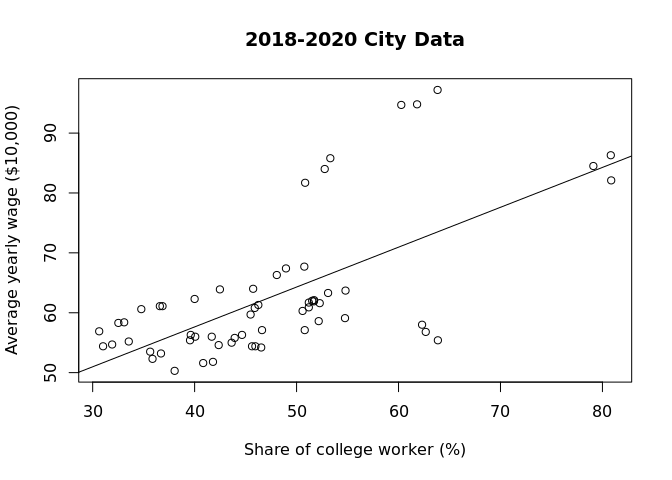
\includegraphics[height=0.5\textheight]{unnamed-chunk-33-1.png}
  \end{center}
  
\end{frame}

\subsection{First Differenced}

\begin{frame}{First Differenced HAC}
    \begin{table}[!htbp] \centering \tiny
        \caption{} 
        \label{} 
        \begin{multicols}{2}
          \begin{tabular}{@{\extracolsep{5pt}}lc} 
            \\[-1.8ex]\hline 
            \hline \\[-1.8ex] 
             & \multicolumn{1}{c}{\textit{Dependent variable:}} \\ 
            \cline{2-2} 
            \\[-1.8ex] & wageDiff \\ 
            \hline \\[-1.8ex] 
             workforceCollegeDiff & $-$0.109 \\ 
              & (0.086) \\ 
              & \\ 
             direct2 & 0.341 \\ 
              & (0.283) \\ 
              & \\ 
             serviceDiff & 0.358$^{***}$ \\ 
              & (0.103) \\ 
              & \\ 
             manufectDiff & $-$0.028 \\ 
              & (0.133) \\ 
              & \\ 
             hiredDiff & $-$0.092 \\ 
              & (0.120) \\ 
              & \\ 
             Constant & 0.671$^{***}$ \\ 
              & (0.141) \\ 
              & \\ 
            \hline \\[-1.8ex] 
          \end{tabular}
          \begin{tabular}{@{\extracolsep{5pt}}lc} \hline \\
            Observations & 40 \\ 
            R$^{2}$ & 0.279 \\ 
            Adjusted R$^{2}$ & 0.173 \\ 
            Residual Std. Error & 0.601 (df = 34) \\ 
            \hline 
            \hline \\[-1.8ex] 
            \textit{Note:}  & \multicolumn{1}{r}{$^{*}$p$<$0.1; $^{**}$p$<$0.05; $^{***}$p$<$0.01} \\ 
            \end{tabular} 
        \end{multicols}
      
      \end{table} 
\end{frame}

\begin{frame}{First Differenced with IV}
    
% Table created by stargazer v.5.2.3 by Marek Hlavac, Social Policy Institute. E-mail: marek.hlavac at gmail.com
% Date and time: Sat, May 21, 2022 - 23:16:07
\begin{table}[!htbp] \centering \tiny
    \caption{} 
    \label{} 
    \begin{multicols}{2}
      \begin{tabular}{@{\extracolsep{5pt}}lc} 
        \\[-1.8ex]\hline 
        \hline \\[-1.8ex] 
         & \multicolumn{1}{c}{\textit{Dependent variable:}} \\ 
        \cline{2-2} 
        \\[-1.8ex] & wageDiff \\ 
        \hline \\[-1.8ex] 
         workforceCollegeDiff & 0.223 \\ 
          & (1.203) \\ 
          & \\ 
         direct2 & 0.294 \\ 
          & (0.433) \\ 
          & \\ 
         serviceDiff & 0.073 \\ 
          & (0.816) \\ 
          & \\ 
         manufectDiff & $-$0.073 \\ 
          & (0.140) \\ 
          & \\ 
         hiredDiff & $-$0.067 \\ 
          & (0.143) \\ 
          & \\ 
         Constant & 0.558 \\ 
          & (0.552) \\ 
          & \\ 
        \hline \\[-1.8ex] 
      \end{tabular}
      \begin{tabular}{@{\extracolsep{5pt}}lc} \hline \\
        Observations & 40 \\ 
        R$^{2}$ & 0.024 \\ 
        Adjusted R$^{2}$ & $-$0.119 \\ 
        Residual Std. Error & 0.748 (df = 34) \\ 
        \hline 
        \hline \\[-1.8ex] 
        \textit{Note:}  & \multicolumn{1}{r}{$^{*}$p$<$0.1; $^{**}$p$<$0.05; $^{***}$p$<$0.01} \\ 
        \end{tabular}
    \end{multicols}
   
  \end{table} 
\end{frame}

\begin{frame}{First Differenced}
  Very large standard error in first differencing estimation may be caused by very small variation in explanatory variable.
  \begin{center}
    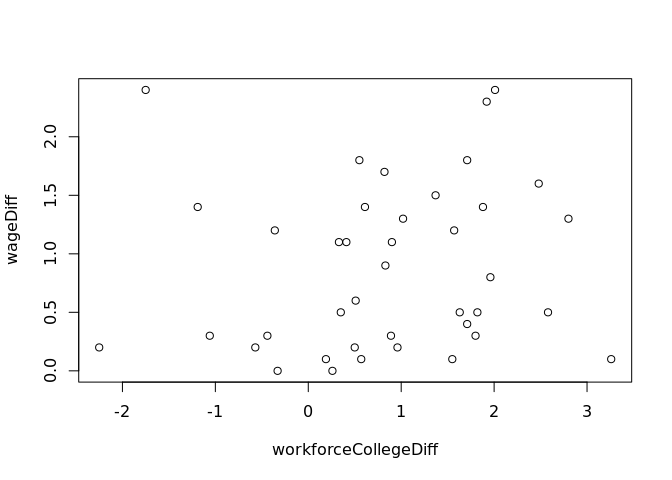
\includegraphics[height=0.5\textheight]{unnamed-chunk-24-1.png}
  \end{center}
  
  So we turned to random effect estimator.
\end{frame}

\subsection{Random Effect}

\begin{frame}{Random Effect}
    % Table created by stargazer v.5.2.3 by Marek Hlavac, Social Policy Institute. E-mail: marek.hlavac at gmail.com
% Date and time: Sat, May 21, 2022 - 23:18:04
\begin{table}[!htbp] \centering \tiny
    \caption{} 
    \label{} 
    \begin{multicols}{2}
      \begin{tabular}{@{\extracolsep{5pt}}lc} 
        \\[-1.8ex]\hline 
        \hline \\[-1.8ex] 
         & \multicolumn{1}{c}{\textit{Dependent variable:}} \\ 
        \cline{2-2} 
        \\[-1.8ex] & wage2018 \\ 
        \hline \\[-1.8ex] 
         workforceCollege\_2018 & 0.403$^{***}$ \\ 
          & (0.114) \\ 
          & \\ 
         manufecture2018 & 0.122 \\ 
          & (0.127) \\ 
          & \\ 
         hired2018 & $-$0.010 \\ 
          & (0.169) \\ 
          & \\ 
         direct & $-$8.666 \\ 
          & (10.479) \\ 
          & \\ 
         directEdu2018 & 0.098 \\ 
          & (0.187) \\ 
          & \\ 
         expensePerCapita2018 & 0.001$^{***}$ \\ 
          & (0.0002) \\ 
          & \\ 
         Constant & 24.754$^{**}$ \\ 
          & (10.832) \\ 
          & \\ 
        \hline \\[-1.8ex] 
      \end{tabular}
      \begin{tabular}{@{\extracolsep{5pt}}lc} \hline \\
        Observations & 60 \\ 
        R$^{2}$ & 0.539 \\ 
        Adjusted R$^{2}$ & 0.487 \\ 
        F Statistic & 62.031$^{***}$ \\ 
        \hline 
        \hline \\[-1.8ex] 
        \textit{Note:}  & \multicolumn{1}{r}{$^{*}$p$<$0.1; $^{**}$p$<$0.05; $^{***}$p$<$0.01} \\ 
        \end{tabular}
    \end{multicols}
  
  \end{table}
\end{frame}

\begin{frame}{RE with IV - First Stage}
  The IV in even less significant here.
    \begin{table}[!htbp] \centering \tiny
        \caption{} 
        \label{} 
      \begin{tabular}{@{\extracolsep{5pt}}lc} 
      \\[-1.8ex]\hline 
      \hline \\[-1.8ex] 
       & \multicolumn{1}{c}{\textit{Dependent variable:}} \\ 
      \cline{2-2} 
      \\[-1.8ex] & workforceCollege\_2018 \\ 
      \hline \\[-1.8ex] 
       workforceYoung\_2013 & 0.082 \\ 
        & (0.584) \\ 
        & \\ 
       Constant & 47.100$^{***}$ \\ 
        & (4.891) \\ 
        & \\ 
      \hline \\[-1.8ex] 
      Observations & 60 \\ 
      R$^{2}$ & 0.0003 \\ 
      Adjusted R$^{2}$ & $-$0.017 \\ 
      F Statistic & 0.020 \\ 
      \hline 
      \hline \\[-1.8ex] 
      \textit{Note:}  & \multicolumn{1}{r}{$^{*}$p$<$0.1; $^{**}$p$<$0.05; $^{***}$p$<$0.01} \\ 
      \end{tabular} 
      \end{table} 
\end{frame}

\begin{frame}{RE with IV - 2SLS}
    \begin{table}[!htbp] \centering \tiny
        \caption{} 
        \label{} 
        \begin{multicols}{2}
          \begin{tabular}{@{\extracolsep{5pt}}lc} 
            \\[-1.8ex]\hline 
            \hline \\[-1.8ex] 
             & \multicolumn{1}{c}{\textit{Dependent variable:}} \\ 
            \cline{2-2} 
            \\[-1.8ex] & wage2018 \\ 
            \hline \\[-1.8ex] 
             workforceCollege\_2018 & 1.776 \\ 
              & (7.636) \\ 
              & \\ 
             manufecture2018 & 0.585 \\ 
              & (2.097) \\ 
              & \\ 
             hired2018 & $-$0.850 \\ 
              & (4.705) \\ 
              & \\ 
             direct & 35.758 \\ 
              & (264.171) \\ 
              & \\ 
             directEdu2018 & $-$0.853 \\ 
              & (5.534) \\ 
              & \\ 
             expensePerCapita2018 & 0.0003 \\ 
              & (0.003) \\ 
              & \\ 
             Constant & 21.315 \\ 
              & (22.243) \\ 
              & \\ 
            \hline \\[-1.8ex] 
          \end{tabular}
          \begin{tabular}{@{\extracolsep{5pt}}lc} \hline \\
            Observations & 60 \\ 
            R$^{2}$ & 0.352 \\ 
            Adjusted R$^{2}$ & 0.279 \\ 
            F Statistic & 17.148$^{***}$ \\ 
            \hline 
            \hline \\[-1.8ex] 
            \textit{Note:}  & \multicolumn{1}{r}{$^{*}$p$<$0.1; $^{**}$p$<$0.05; $^{***}$p$<$0.01} \\ 
            \end{tabular} 
        \end{multicols}
      
      \end{table}
\end{frame}

\begin{frame}{Takeaways}
  \begin{itemize}
    \item Random effect estimation gives a larger significant coefficient than cross sectional OLS.
    \item IV using RE also suggest a even larger causal effect.
  \end{itemize}
  
\end{frame}

\begin{frame}{Other Panel Data Methods}
  \begin{itemize}
    \item We find Fixed Effect results vary similar to RE. This can also be seen by the close to one $\hat{\theta}$.
    \item Pooling independent method finds only the effect of industry structure, $manufecture2018$, has a significant coefficient of 0.4280. 
  \end{itemize}
  \begin{table}[]
    \begin{tabular}{llll}
                  & var     & std.dev & share \\
    idiosyncratic & 0.5627  & 0.7501  & 0.015 \\
    individual    & 37.9300 & 6.1587  & 0.985 \\ \hline \\[-1.8ex]
    $\hat{\theta}$= 0.9299 &         &         &      
    \end{tabular}
    \caption{Random effect estimation (without IV)}
    \label{tab: REeffect}
    \end{table}
\end{frame}

\begin{frame}{Remarks}
  \begin{itemize}
    \item Our panel data analysis requires strict exogeneity, for which we kind of take it for granted.
    \item The $R^2$ in our RE estimation is only 0.487, which definitely leaves room for improvement.
  \end{itemize}
  
\end{frame}

\section[Time Series]{1982-2020 Time Series Data}
\begin{frame}{Data}
  \begin{itemize}
    \item Between 1982-2020
    \item National data
    \item Due to data limitation, after some test we decided to choose:
    \begin{itemize}
      \item \textbf{Average household income} ($income_t$) as the dependent variable.
      \item \textbf{Government education budget} ($edufund_t$) as the main explanatory variable.
    \end{itemize}
  \end{itemize}
\end{frame}

\begin{frame}{Autoregression}
  \begin{itemize}
    \item We find $income_t$ and $income_{t-1}$ to be highly correlated with 0.9975 correlation.
    \item So we perform first differencing on all variable and define
    \begin{equation}
      cincome_t = income_t - income_{t-1}
    \end{equation}
  \end{itemize}
\end{frame}

\subsection{Model 1}

\begin{frame}{Model 1 Specification}
  \begin{multline}
    cincome = cincome\_lag + cedufund + cunem \\ + cindpd + cavgGDP
  \end{multline}
  \begin{itemize}
    \item $cincome\_lag$ in a 2 periods lag term of the dependent.
    \item $cedufund$ is our main explanatory.
    \item $cunem$ refers to unemployment rate.
    \item $cindpd$ is the gross production of manufecturing industry, in million NTD.
    \item $cavgGDP$ is the average GDP per capita.
  \end{itemize}
\end{frame}

\begin{frame}{Model 1 Results}
  % Table created by stargazer v.5.2.3 by Marek Hlavac, Social Policy Institute. E-mail: marek.hlavac at gmail.com
% Date and time: Sun, May 22, 2022 - 23:12:06
\begin{table}[!htbp] \centering \tiny
  \caption{First Differenced MLR} 
  \label{tab: FDMLR} 
  \begin{multicols}{2}
\begin{tabular}{@{\extracolsep{5pt}}lc} 
\\[-1.8ex]\hline 
\hline \\[-1.8ex] 
 & \multicolumn{1}{c}{\textit{Dependent variable:}} \\ 
\cline{2-2} 
\\[-1.8ex] & cincome[3:38] \\ 
\hline \\[-1.8ex] 
 cincome$\_$lag & 0.555$^{***}$ \\ 
  & (0.121) \\ 
  & \\ 
 cedufund[3:38] & 0.0001$^{**}$ \\ 
  & (0.00003) \\ 
  & \\ 
 cunem[3:38] & $-$8,050.278$^{***}$ \\ 
  & (1,597.252) \\ 
  & \\ 
 cindpd[3:38] & $-$0.001 \\ 
  & (0.001) \\ 
  & \\ 
 cavgGDP[3:38] & 0.149$^{**}$ \\ 
  & (0.061) \\ 
  & \\ 
 Constant & 178.333 \\ 
  & (1,437.168) \\ 
  & \\
      \hline \\[-1.8ex] 
    \end{tabular}
    \begin{tabular}{@{\extracolsep{5pt}}lc} \hline \\
      Observations & 36 \\ 
R$^{2}$ & 0.744 \\ 
Adjusted R$^{2}$ & 0.702 \\ 
Residual Std. Error & 3,445.707 (df = 30) \\ 
F Statistic & 17.451$^{***}$ (df = 5; 30) \\ 
      \hline 
      \hline \\[-1.8ex] 
      \textit{Note:}  & \multicolumn{1}{r}{$^{*}$p$<$0.1; $^{**}$p$<$0.05; $^{***}$p$<$0.01} \\ 
      \end{tabular} 
  \end{multicols}

\end{table}
\end{frame}

\begin{frame}{Serial Correlation}
  Define $u_t$ as the residuals of the previous model.
  % Table created by stargazer v.5.2.3 by Marek Hlavac, Social Policy Institute. E-mail: marek.hlavac at gmail.com
% Date and time: Thu, May 26, 2022 - 16:46:48
\begin{table}[!htbp] \centering \tiny
  \caption{} 
  \label{} 
\begin{tabular}{@{\extracolsep{5pt}}lc} 
\\[-1.8ex]\hline 
\hline \\[-1.8ex] 
 & \multicolumn{1}{c}{\textit{Dependent variable:}} \\ 
\cline{2-2} 
\\[-1.8ex] & ut \\ 
\hline \\[-1.8ex] 
 ut\_1 & 0.023 \\ 
  & (0.194) \\ 
  & \\ 
 Constant & $-$52.015 \\ 
  & (553.908) \\ 
  & \\ 
\hline \\[-1.8ex] 
Observations & 35 \\ 
R$^{2}$ & 0.0004 \\ 
Adjusted R$^{2}$ & $-$0.030 \\ 
Residual Std. Error & 3,265.292 (df = 33) \\ 
F Statistic & 0.014 (df = 1; 33) \\ 
\hline 
\hline \\[-1.8ex] 
\textit{Note:}  & \multicolumn{1}{r}{$^{*}$p$<$0.1; $^{**}$p$<$0.05; $^{***}$p$<$0.01} \\ 
\end{tabular} 
\end{table} 
Our model doesn't seem to be affected by SC.
\end{frame}

\begin{frame}{Heteroskedasticity}
  Breusch-Pagan test:

  BP = 5.4892, df = 5, p-value = 0.3591

Our model doesn't seem to be affected by heteroskedasticity.
\end{frame}

\subsection{Model 2}

\begin{frame}{Model 2 Specification}
  \begin{multline}
    cincome = cincome\_lag + cedufund + cunem + cindpd \\
    + cindpd\_lag + cavgGDP
  \end{multline}
  \begin{itemize}
    \item $cincome\_lag$ is a 2 periods lag term of the dependent.
    \item $cedufund$ is our main explanatory.
    \item $cunem$ refers to unemployment rate.
    \item $cindpd$ is the gross production of manufecturing industry, in million NTD.
    \item $cindpd\_lag$ is a 1 period lag term of $cindpd$.
    \item $cavgGDP$ is the average GDP per capita.
  \end{itemize}
\end{frame}

\begin{frame}{Model 2 Results}
  % Table created by stargazer v.5.2.3 by Marek Hlavac, Social Policy Institute. E-mail: marek.hlavac at gmail.com
% Date and time: Sun, May 22, 2022 - 23:12:06
\begin{table}[!htbp] \centering \tiny
  \caption{First Differenced MLR model 2} 
  \label{tab: FDMLR2} 
  \begin{multicols}{2}
  \begin{tabular}{@{\extracolsep{5pt}}lc} 
    \\[-1.8ex]\hline 
    \hline \\[-1.8ex] 
     & \multicolumn{1}{c}{\textit{Dependent variable:}} \\ 
    \cline{2-2} 
    \\[-1.8ex] & cincome[3:38] \\ 
    \hline \\[-1.8ex] 
     cincome$\_$lag & 0.553$^{***}$ \\ 
      & (0.112) \\ 
      & \\ 
     cedufund[3:38] & 0.0001$^{***}$ \\ 
      & (0.00003) \\ 
      & \\ 
     cunem[3:38] & $-$9,850.055$^{***}$ \\ 
      & (1,643.410) \\ 
      & \\ 
     cindpd[3:38] & $-$0.001$^{*}$ \\ 
      & (0.001) \\ 
      & \\ 
     cindpd$\_$lag & $-$0.001$^{**}$ \\ 
      & (0.001) \\ 
      & \\ 
      \hline \\[-1.8ex] 
    \end{tabular}
    \begin{tabular}{@{\extracolsep{5pt}}lc} \hline \\
      cavgGDP[3:38] & 0.077 \\ 
  & (0.063) \\ 
  & \\ 
 Constant & 2,159.014 \\ 
  & (1,548.312) \\ 
  & \\ 
\hline \\[-1.8ex] 
Observations & 36 \\ 
R$^{2}$ & 0.789 \\ 
Adjusted R$^{2}$ & 0.745 \\ 
Residual Std. Error & 3,182.269 (df = 29) \\ 
F Statistic & 18.079$^{***}$ (df = 6; 29) \\ 
      \hline 
      \hline \\[-1.8ex] 
      \textit{Note:}  & \multicolumn{1}{r}{$^{*}$p$<$0.1; $^{**}$p$<$0.05; $^{***}$p$<$0.01} \\ 
      \end{tabular} 
  \end{multicols}

\end{table}
\end{frame}

\begin{frame}{Serial Correlation}
  Define $u_t$ as the residuals of the previous model.
  % Table created by stargazer v.5.2.3 by Marek Hlavac, Social Policy Institute. E-mail: marek.hlavac at gmail.com
% Date and time: Thu, May 26, 2022 - 16:51:16
\begin{table}[!htbp] \centering \tiny
  \caption{} 
  \label{} 
\begin{tabular}{@{\extracolsep{5pt}}lc} 
\\[-1.8ex]\hline 
\hline \\[-1.8ex] 
 & \multicolumn{1}{c}{\textit{Dependent variable:}} \\ 
\cline{2-2} 
\\[-1.8ex] & ut \\ 
\hline \\[-1.8ex] 
 ut\_1 & 0.019 \\ 
  & (0.198) \\ 
  & \\ 
 Constant & $-$43.651 \\ 
  & (503.820) \\ 
  & \\ 
\hline \\[-1.8ex] 
Observations & 35 \\ 
R$^{2}$ & 0.0003 \\ 
Adjusted R$^{2}$ & $-$0.030 \\ 
Residual Std. Error & 2,967.877 (df = 33) \\ 
F Statistic & 0.009 (df = 1; 33) \\ 
\hline 
\hline \\[-1.8ex] 
\textit{Note:}  & \multicolumn{1}{r}{$^{*}$p$<$0.1; $^{**}$p$<$0.05; $^{***}$p$<$0.01} \\ 
\end{tabular} 
\end{table}
Our model doesn't seem to be affected by SC.
\end{frame}

\begin{frame}{Heteroskedasticity}
  Breusch-Pagan test:

  BP = 5.3746, df = 6, p-value = 0.4967

Our model doesn't seem to be affected by heteroskedasticity.
\end{frame}

\subsection{Model 3}

\begin{frame}{Model 3 Specification}
  \begin{multline}
    cincome = cincome\_lag + cedufund + cunem \\
    + cservpd + cavgGDP
  \end{multline}
  \begin{itemize}
    \item $cincome\_lag$ in a 2 periods lag term of the dependent.
    \item $cedufund$ is our main explanatory.
    \item $cunem$ refers to unemployment rate.
    \item $cservpd$ is the gross production of service industry, in million NTD.
    \item $cavgGDP$ is the average GDP per capita.
  \end{itemize}
\end{frame}

\begin{frame}{Model 3 Results}
  % Table created by stargazer v.5.2.3 by Marek Hlavac, Social Policy Institute. E-mail: marek.hlavac at gmail.com
% Date and time: Sun, May 22, 2022 - 23:12:06
\begin{table}[!htbp] \centering \tiny
  \caption{First Differenced MLR model 3} 
  \label{tab: FDMLR3} 
  \begin{multicols}{2}
  \begin{tabular}{@{\extracolsep{5pt}}lc} 
    \\[-1.8ex]\hline 
    \hline \\[-1.8ex] 
     & \multicolumn{1}{c}{\textit{Dependent variable:}} \\ 
    \cline{2-2} 
    \\[-1.8ex] & cincome[3:38] \\ 
    \hline \\[-1.8ex] 
     cincome$\_$lag & 0.729$^{***}$ \\ 
      & (0.126) \\ 
      & \\ 
     cedufund[3:38] & 0.0001$^{**}$ \\ 
      & (0.00003) \\ 
      & \\ 
     cunem[3:38] & $-$9,225.299$^{***}$ \\ 
      & (1,609.773) \\ 
      & \\ 
     cservpd[3:38] & $-$0.009$^{**}$ \\ 
      & (0.004) \\ 
      & \\ 
     cavgGDP[3:38] & 0.201$^{***}$ \\ 
      & (0.063) \\ 
      & \\ 
     Constant & 1,517.859 \\ 
      & (1,488.989) \\ 
      & \\ 
    \end{tabular}
    \begin{tabular}{@{\extracolsep{5pt}}lc} \hline \\
      Observations & 36 \\ 
R$^{2}$ & 0.774 \\ 
Adjusted R$^{2}$ & 0.737 \\ 
Residual Std. Error & 3,235.215 (df = 30) \\ 
F Statistic & 20.602$^{***}$ (df = 5; 30) \\ 
      \hline 
      \hline \\[-1.8ex] 
      \textit{Note:}  & \multicolumn{1}{r}{$^{*}$p$<$0.1; $^{**}$p$<$0.05; $^{***}$p$<$0.01} \\ 
      \end{tabular} 
  \end{multicols}

\end{table}
\end{frame}
\begin{frame}{Serial Correlation}
  Define $u_t$ as the residuals of the previous model.
  % Table created by stargazer v.5.2.3 by Marek Hlavac, Social Policy Institute. E-mail: marek.hlavac at gmail.com
% Date and time: Thu, May 26, 2022 - 16:54:27
\begin{table}[!htbp] \centering \tiny
  \caption{} 
  \label{} 
\begin{tabular}{@{\extracolsep{5pt}}lc} 
\\[-1.8ex]\hline 
\hline \\[-1.8ex] 
 & \multicolumn{1}{c}{\textit{Dependent variable:}} \\ 
\cline{2-2} 
\\[-1.8ex] & ut \\ 
\hline \\[-1.8ex] 
 ut\_1 & 0.119 \\ 
  & (0.181) \\ 
  & \\ 
 Constant & $-$19.639 \\ 
  & (517.243) \\ 
  & \\ 
\hline \\[-1.8ex] 
Observations & 35 \\ 
R$^{2}$ & 0.013 \\ 
Adjusted R$^{2}$ & $-$0.017 \\ 
Residual Std. Error & 3,055.879 (df = 33) \\ 
F Statistic & 0.435 (df = 1; 33) \\ 
\hline 
\hline \\[-1.8ex] 
\textit{Note:}  & \multicolumn{1}{r}{$^{*}$p$<$0.1; $^{**}$p$<$0.05; $^{***}$p$<$0.01} \\ 
\end{tabular} 
\end{table} 
Our model doesn't seem to be affected by SC.
\end{frame}

\begin{frame}{Heteroskedasticity}
  Breusch-Pagan test:

  BP = 10.115, df = 5, p-value = 0.07205

Our model doesn't seem to be affected by heteroskedasticity.
\end{frame}

\begin{frame}{Takeaways}
  \begin{itemize}
    \item All 3 models yields similar results.
    \item Government education budget has a positive, significant, but small effect.
    \item The models are free from heteroskedasticity and serial correlation.
    \item $R^2$s lies in the 0.7 range, still room for improvement.
    \item The main explanatory accounts for all education level, not just higher.
    \item The dependent also doesn't directly indicate wage.
  \end{itemize}
\end{frame}

\begin{frame}{Comparisons}
  In comparison to our cross sectional analysis,
  \begin{itemize}
    \item TS obtains smaller coefficient,
    \item TS models have lower $R^2$.
  \end{itemize}
  In comparison to our panel analysis,
  \begin{itemize}
    \item TS obtains smaller coefficient,
    \item TS models have higher $R^2$.
  \end{itemize}
  From several models using cross section, panel, time series methods, we find (higher)education does have a positive effect
  on average wage. How much the effect is distributed to the external is beyond the scope of this work.
\end{frame}

\subsection{Detrending}
\begin{frame}{Detrending MLR}
  % Table created by stargazer v.5.2.3 by Marek Hlavac, Social Policy Institute. E-mail: marek.hlavac at gmail.com
% Date and time: Sun, May 22, 2022 - 23:17:45
\begin{table}[!htbp] \centering \tiny
  \caption{} 
  \label{} 
  \begin{multicols}{2}
    \begin{tabular}{@{\extracolsep{5pt}}lc} 
      \\[-1.8ex]\hline 
      \hline \\[-1.8ex] 
       & \multicolumn{1}{c}{\textit{Dependent variable:}} \\ 
      \cline{2-2} 
      \\[-1.8ex] & income \\ 
      \hline \\[-1.8ex] 
       edufund & 0.0003$^{***}$ \\ 
        & (0.00002) \\ 
        & \\ 
       unem & $-$4,634.824$^{***}$ \\ 
        & (1,311.579) \\ 
        & \\ 
       indpd & $-$0.004$^{***}$ \\ 
        & (0.001) \\ 
        & \\ 
       avgGDP & 0.275$^{***}$ \\ 
        & (0.066) \\ 
        & \\ 
       t & $-$2,095.528 \\ 
        & (1,398.582) \\ 
        & \\ 
       Constant & 32,611.320$^{***}$ \\ 
        & (5,618.118) \\ 
        & \\ 
      \hline \\[-1.8ex] 
    \end{tabular}
      \begin{tabular}{@{\extracolsep{5pt}}lc} \hline \\
      Observations & 39 \\ 
      R$^{2}$ & 0.996 \\ 
      Adjusted R$^{2}$ & 0.995 \\ 
      Residual Std. Error & 6,269.286 (df = 33) \\ 
      F Statistic & 1,575.655$^{***}$ (df = 5; 33) \\ 
      \hline 
      \hline \\[-1.8ex] 
      \textit{Note:}  & \multicolumn{1}{r}{$^{*}$p$<$0.1; $^{**}$p$<$0.05; $^{***}$p$<$0.01} \\ 
      \end{tabular} 
  \end{multicols}

\end{table} 
\end{frame}

\begin{frame}{Detrended AR}
  First, we obtain the detrended variables $\ddot{y_t}$ by regressing
  \begin{equation}
    y_t=\alpha_0+\alpha_1 t+e_t
  \end{equation}
  and specify $\ddot{y_t}=e_t$.

  Subsequently, we found detrended $\ddot{income_t}$ highly correlated to $\ddot{income_{t-1}}$ with correlation 0.9570.
  
  So we performed first differencing and define
  \begin{equation}
    cincome\_ dt_t=\ddot{income_t}-\ddot{income_{t-1}}
  \end{equation}
\end{frame}

\begin{frame}{FD Detrending MLR}
  Then the regression result is \textbf{exactly the same} as the non-detrending FD MLR (in table \ref{tab: FDMLR}).
  % Table created by stargazer v.5.2.3 by Marek Hlavac, Social Policy Institute. E-mail: marek.hlavac at gmail.com
% Date and time: Sun, May 22, 2022 - 23:28:09
\begin{table}[!htbp] \centering \tiny
  \caption{First differenced detrending MLR} 
  \label{} 
  \begin{multicols}{2}
    \begin{tabular}{@{\extracolsep{5pt}}lc} 
      \\[-1.8ex]\hline 
      \hline \\[-1.8ex] 
       & \multicolumn{1}{c}{\textit{Dependent variable:}} \\ 
      \cline{2-2} 
      \\[-1.8ex] & cincome\_dt[4:38] \\ 
      \hline \\[-1.8ex] 
       cincome$\_$dt[2:36] & 0.558$^{***}$ \\ 
        & (0.122) \\ 
        & \\ 
       cedufund\_dt[4:38] & 0.0001$^{**}$ \\ 
        & (0.00003) \\ 
        & \\ 
       cunem\_dt[4:38] & $-$8,154.249$^{***}$ \\ 
        & (1,623.290) \\ 
        & \\ 
       cindpd$\_$dt[4:38] & $-$0.001 \\ 
        & (0.001) \\ 
        & \\ 
       cavgGDP\_dt[4:38] & 0.154$^{**}$ \\ 
        & (0.062) \\ 
        & \\ 
       Constant & 152.261 \\ 
        & (602.216) \\ 
      \end{tabular}
      \begin{tabular}{@{\extracolsep{5pt}}lc}  
      \hline \\[-1.8ex] 
      Observations & 35 \\ 
      R$^{2}$ & 0.741 \\ 
      Adjusted R$^{2}$ & 0.696 \\ 
      Residual Std. Error & 3,482.437 (df = 29) \\ 
      F Statistic & 16.602$^{***}$ (df = 5; 29) \\ 
      \hline 
      \hline \\[-1.8ex] 
      \textit{Note:}  & \multicolumn{1}{r}{$^{*}$p$<$0.1; $^{**}$p$<$0.05; $^{***}$p$<$0.01} \\ 
      \end{tabular} 
  \end{multicols}

\end{table}
\end{frame}

\begin{frame}{SC, Heteroskedasticity and Our Question}
  \begin{itemize}
    \item Serial correlation and heteroskedasticity result are also the same.
    \item So, is detrending redundant after first-differencing?
  \end{itemize}

\end{frame}

\begin{frame}[allowframebreaks]{Reference}
  \printbibliography
\end{frame}

\end{document}